\documentclass{article}
\usepackage[utf8]{inputenc}

\title{EE568 Project 3 - PM Motor Comparison Analysis}
\author{by Hakan Saraç - 2408086}
\date{}



\usepackage{natbib}
\usepackage{graphicx}
\usepackage{indentfirst}
\usepackage{siunitx}
\usepackage{svg}
\usepackage{hyperref}
\usepackage{amsmath, bm}
\usepackage{graphicx} 
\usepackage{pstool}

\addtolength{\oddsidemargin}{-.875in}
\addtolength{\evensidemargin}{-.875in}
\addtolength{\textwidth}{1.75in}
\addtolength{\topmargin}{-.875in}
\addtolength{\textheight}{1.75in}    
\begin{document}

\maketitle

\newpage
\section{Introduction}
In this project, we will examined some stuff.

\section{Question 1 - Magnetic Loading}
\subsection{Part - a}

Flux path for one pole pair is provided in Figure \ref{fig:FluxPath} and the corresponding equivalent magnetic circuit is provided in Figure \ref{fig:MagneticCircuit}. In this part, the permeability of the rotor and stator are assumed to be infinite. Therefore, the reluctance of core material becomes zero. Another assumption can be made as that there is no fringing or leakage flux and flux lines are straight as shown in Figure \ref{fig:FluxPath} with green lines. \newline
The machine parameters are as follows:
\begin{itemize}
    \item Number Of Poles: 4
    \item Motor Axial Length: 100 mm
    \item Air Gap Clearance: 1 mm
    \item Magnet To Pole Pitch Ratio: 0.8
    \item Rotor Diameter: 100 mm
    \item Magnet Thickness: 4 mm
    \item Magnet Type: NdFeB N42 grade (ur=1.05), radial shaped
\end{itemize} 
\bigskip
\noindent With the assumptions made, the reluctance $R_{m1}$ and $R_{m2}$ in Figure \ref{fig:FluxPath} can be calculated as:

\begin{equation} \label{eqn:PoleAreaFormula}
    A_{pole} = \frac{\pi \: D_i \: L_{axial}}{P}=0.007853 \: \mathrm{m^2}
\end{equation}
where P is the number of poles.

\bigskip


\noindent From the magnet to pole pitch ratio value of 0.8 (shown as $K$ in (\ref{eqn:MagnetAreaPerPole})), the magnet area per pole can be calculated. 
\bigskip

\begin{equation} \label{eqn:MagnetAreaPerPole}
    A_{magnetperpole} = A_{pole}\cdot K = 0.006283 \: \mathrm{m^2}
\end{equation}

\begin{equation} \label{eqn:NonMagnetAreaPerPole}
    A_{nonmagnetperpole} = (1-K) \cdot A_{pole} = 0.00157 \: \mathrm{m^2}
\end{equation}

\begin{equation} \label{eqn:MagnetReluctance}
    R_{m1}  =  R_{m2} =  \frac{H_{magnet}}{A_{magnetperpole} \cdot \mu_0 \cdot \mu_r}  = 482480 \: \mathrm{\frac{1}{Henry}} 
\end{equation}

\begin{equation} \label{eqn:MagnetReluctance}
    R_{ag1}  =  R_{ag2} =  \frac{H_{airgap}}{A_{magnetperpole} \cdot \mu_0}  =  126650  \: \mathrm{\frac{1}{Henry}} 
\end{equation}

\begin{equation} \label{eqn:MmfPerMagnet}
    \mathcal{F}_{permagnet} = A_{magnetperpole} \cdot B_{residual} \cdot R_{m1} = 4001.61 \: \mathrm{Amperes}
\end{equation}

\bigskip

\noindent Assuming that the core is infinitely permeable, loop equation of the equivalent circuit (see Fig.\ref{fig:MagneticCircuit}) results in (\ref{eqn:AirGapFlux}).
\bigskip

\begin{equation} \label{eqn:AirGapFlux}
    \phi_{m} = \frac{2 \cdot \mathcal{F}_{permagnet}}{R_{m1}+R_{m2}+R_{ag1}+R_{ag2}} = 6.57 \: \mathrm{mWeber}
\end{equation}

\begin{equation} \label{eqn:AirGapFluxDensity}
    B_{m} = \frac{\phi_{m}}{A_{magnetperpole}} = 1.0455 \: \mathrm{Tesla}
\end{equation}
However, the FEA simulations gave a peak flux density value of $1.0174\: \mathrm{T} $ while the analytical calculations are $ 1.0455  \: \mathrm{T}$. The difference is due to the leakage flux. 

\noindent From the values found in (\ref{eqn:AirGapFluxDensity}), the magnetic field strength value is provided in (\ref{eqn:MagneticFieldStrength}).
\begin{equation} \label{eqn:MagneticFieldStrength}
    H_m = \frac{B_m-B_{residual}}{\mu_r \cdot \mu_0} = -208004.48 \: \mathrm{\frac{A}{m}}
\end{equation}

As stated in \cite{e-magnetsuk}, the coercivity value for a N42 NdFeB magnet is around $\pmb{955} \: \pmb{\mathrm{\frac{kA}{m}}}$

\subsection{Part - b}
The magnetic loading of the machine is given in (\ref{eqn:MagneticLoading})
\begin{equation} \label{eqn:MagneticLoading}
    \bar{B} = \frac{P\:\phi_{m}}{\pi \: D_i \: L_{axial}} = 0.8364 \: \mathrm{Tesla}
\end{equation}

\subsection{Part - c}
The FEA results are provided in Figure \ref{fig:MagB}.
\begin{figure}[h!]
\centering
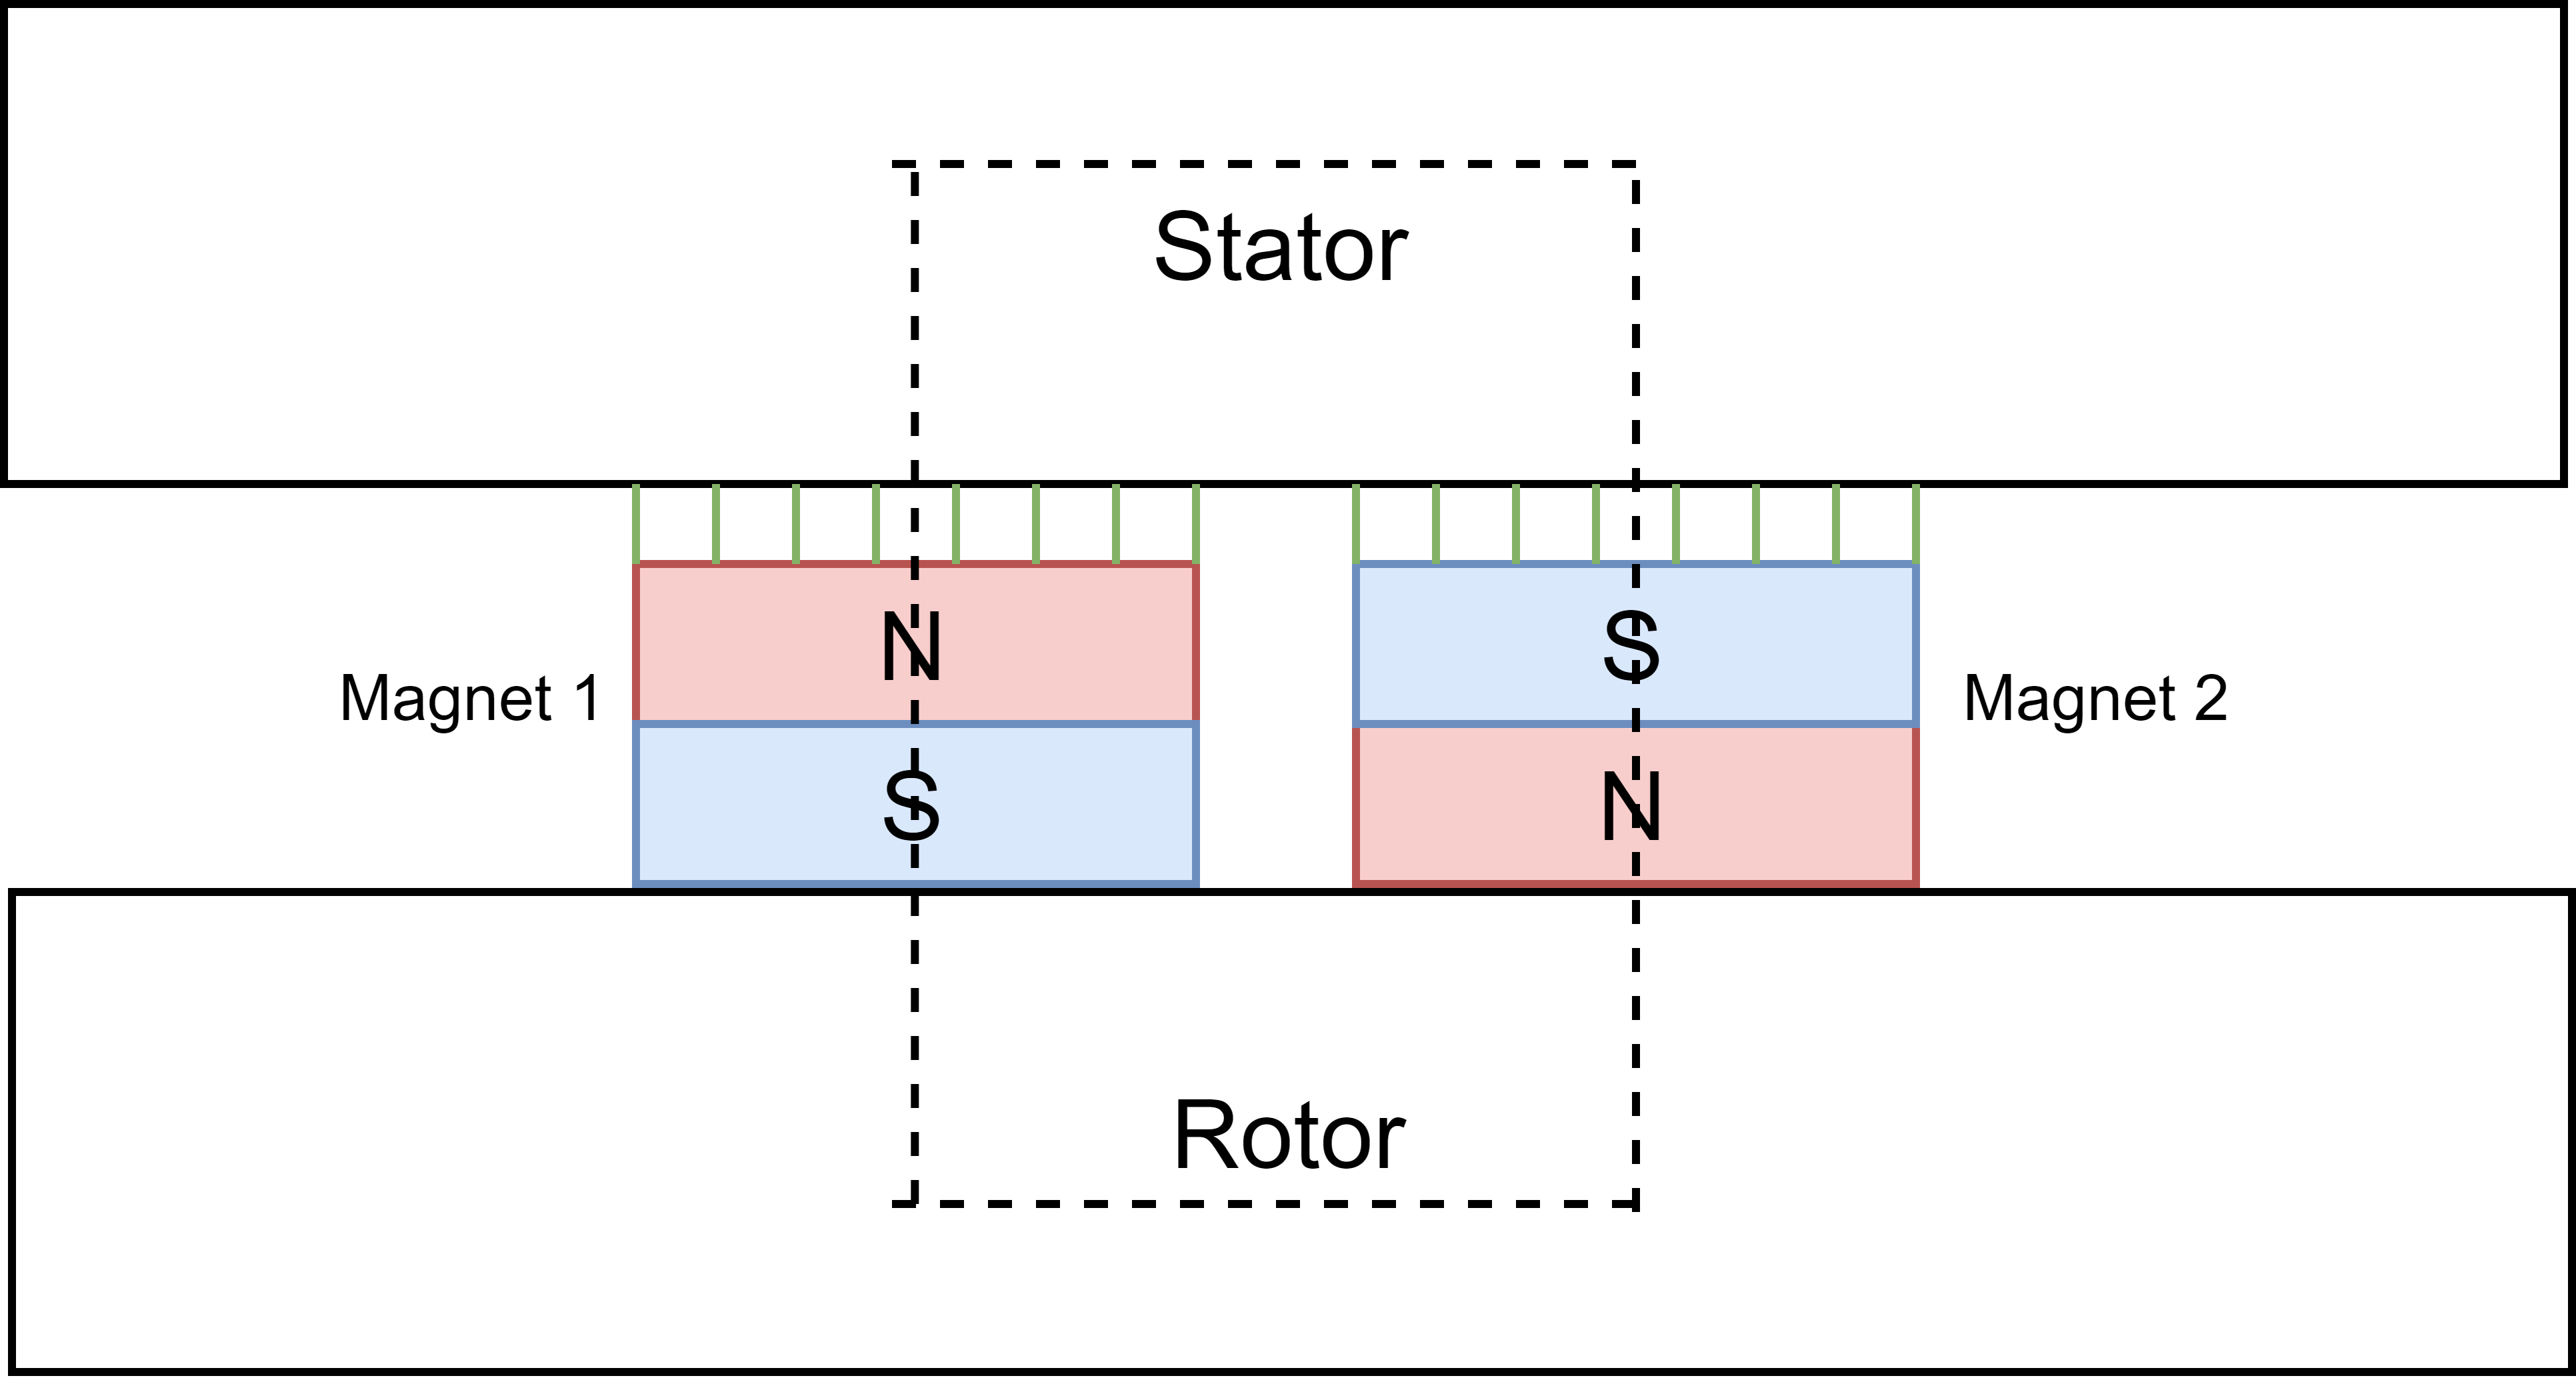
\includegraphics[scale=1.2]{Figures/FluxPath.png}
\caption{Flux Path Through a Pole Pair }
\label{fig:FluxPath}
\end{figure}


\begin{figure}[h!]
\centering
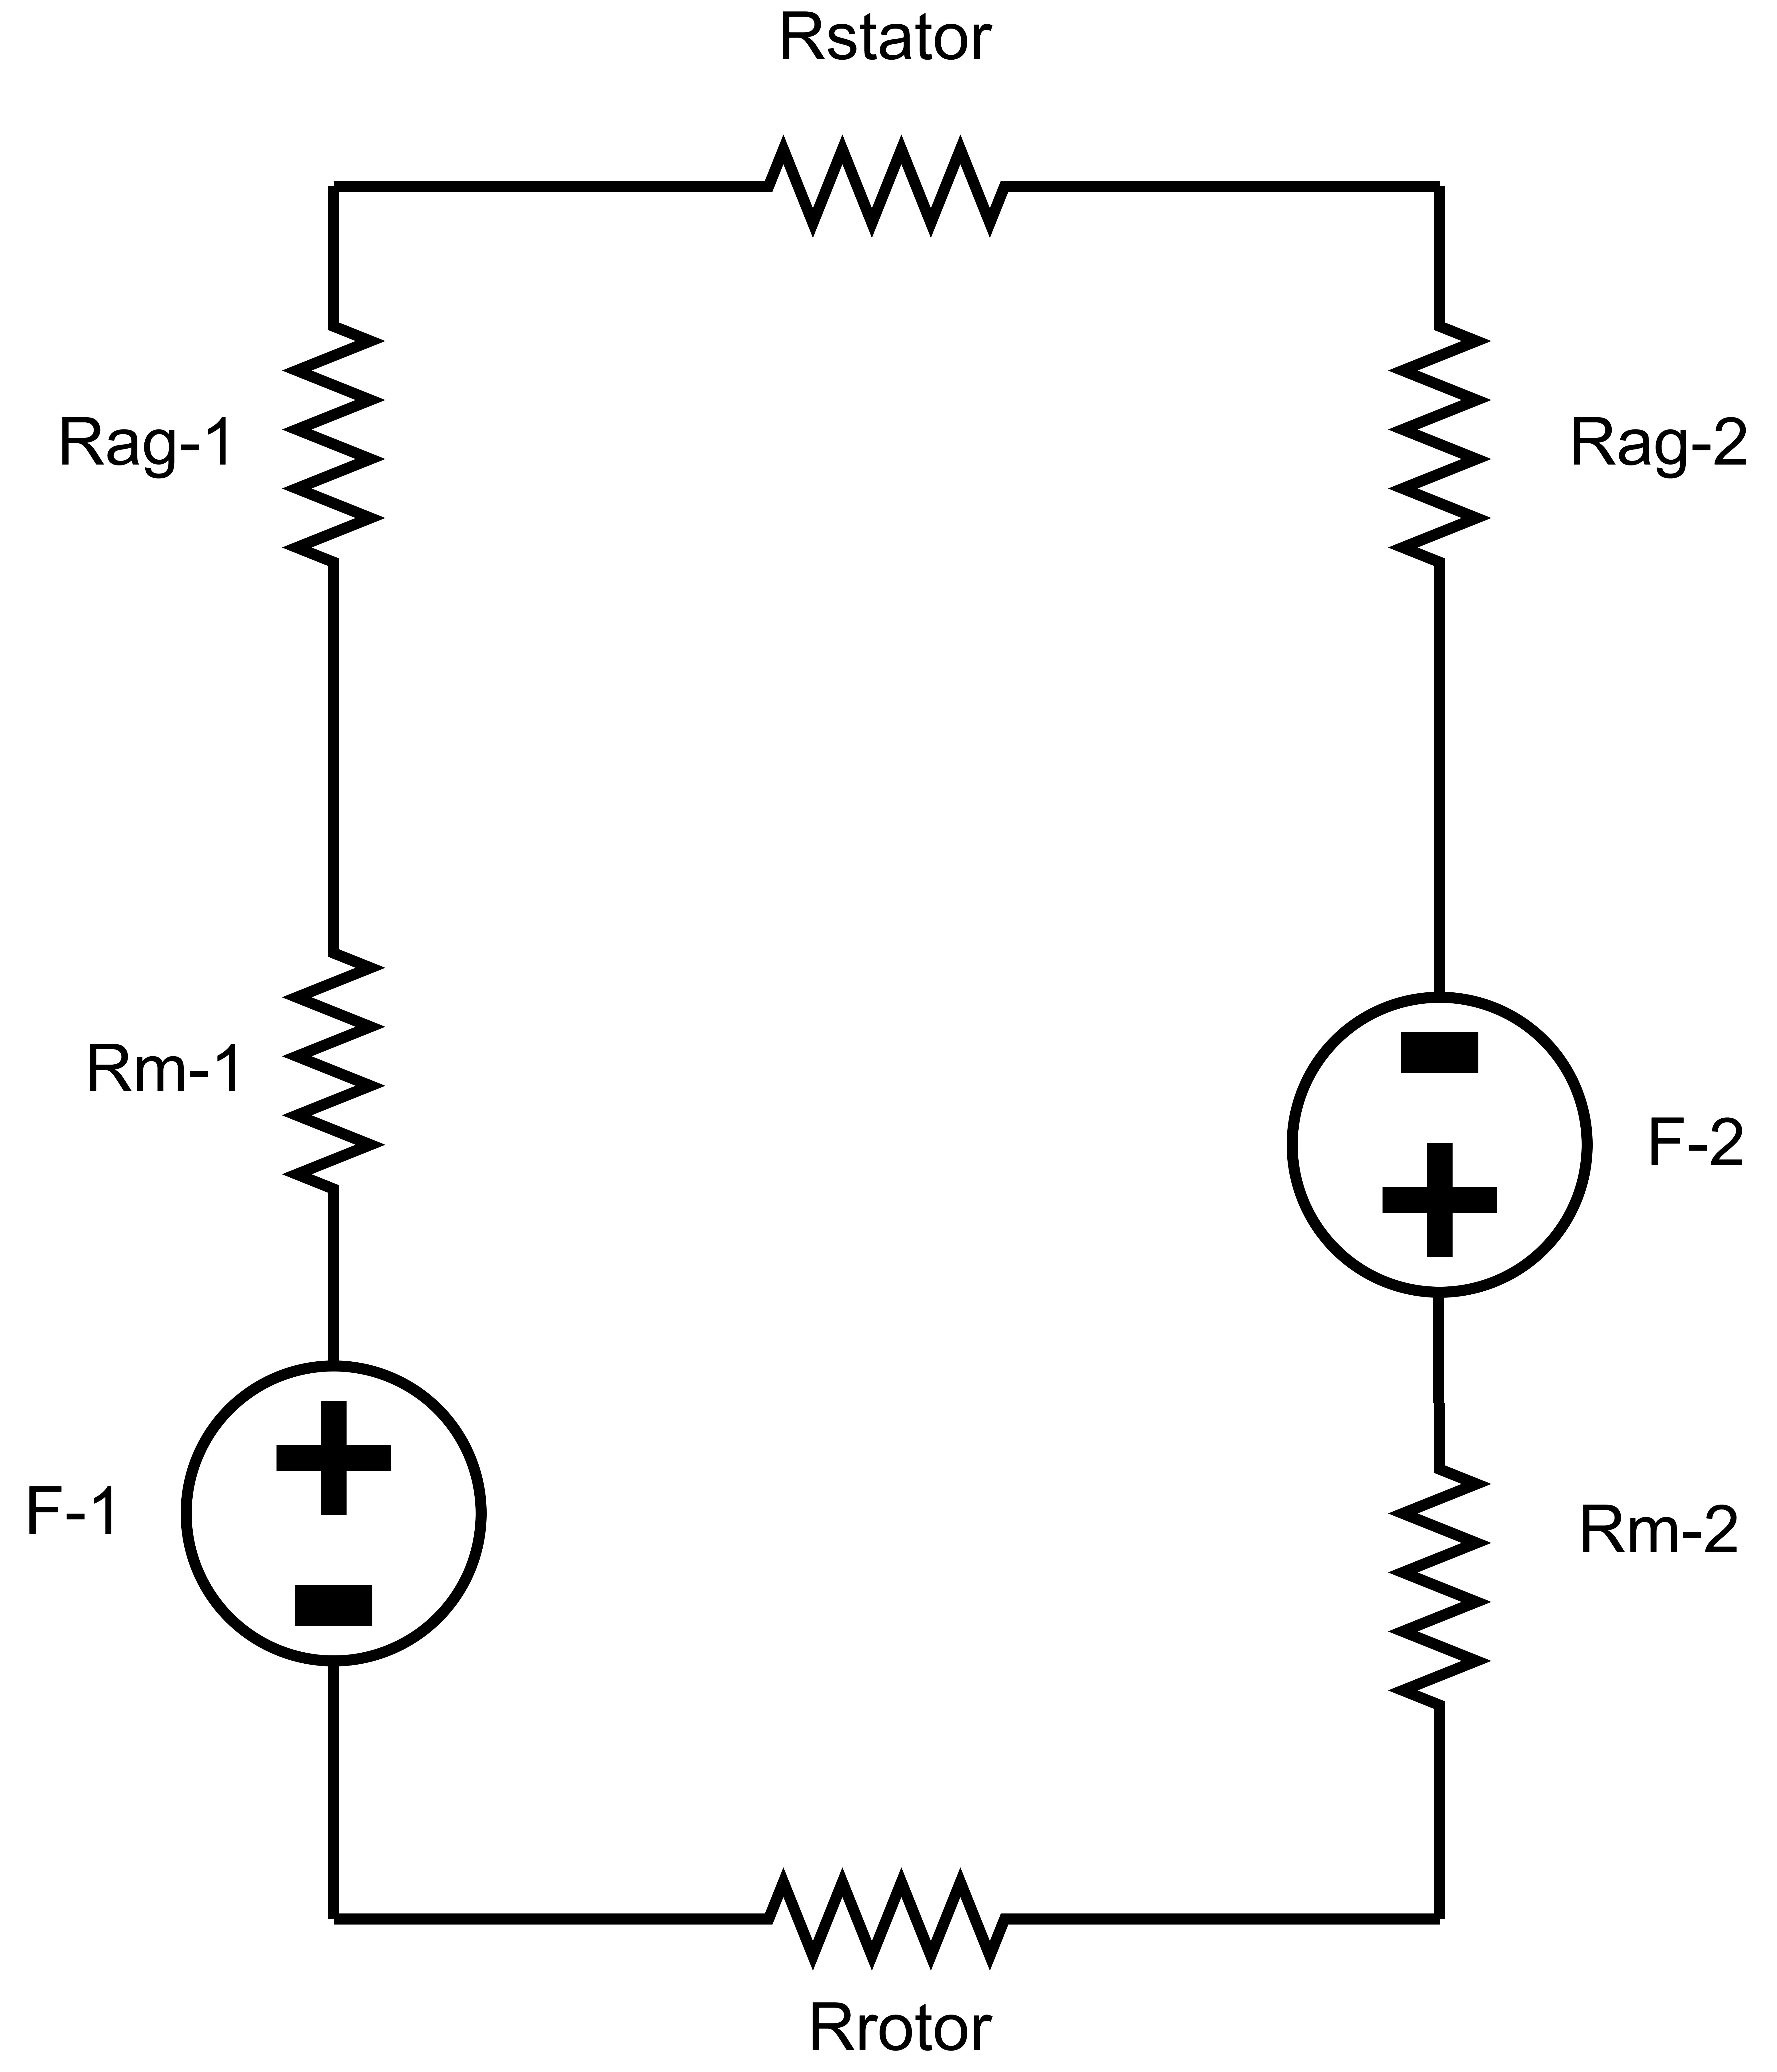
\includegraphics[scale=0.5]{Figures/MagneticCircuit.png}
\caption{Magnetic Equivalent Circuit }
\label{fig:MagneticCircuit}
\end{figure}
\begin{figure}[h!]
\centering
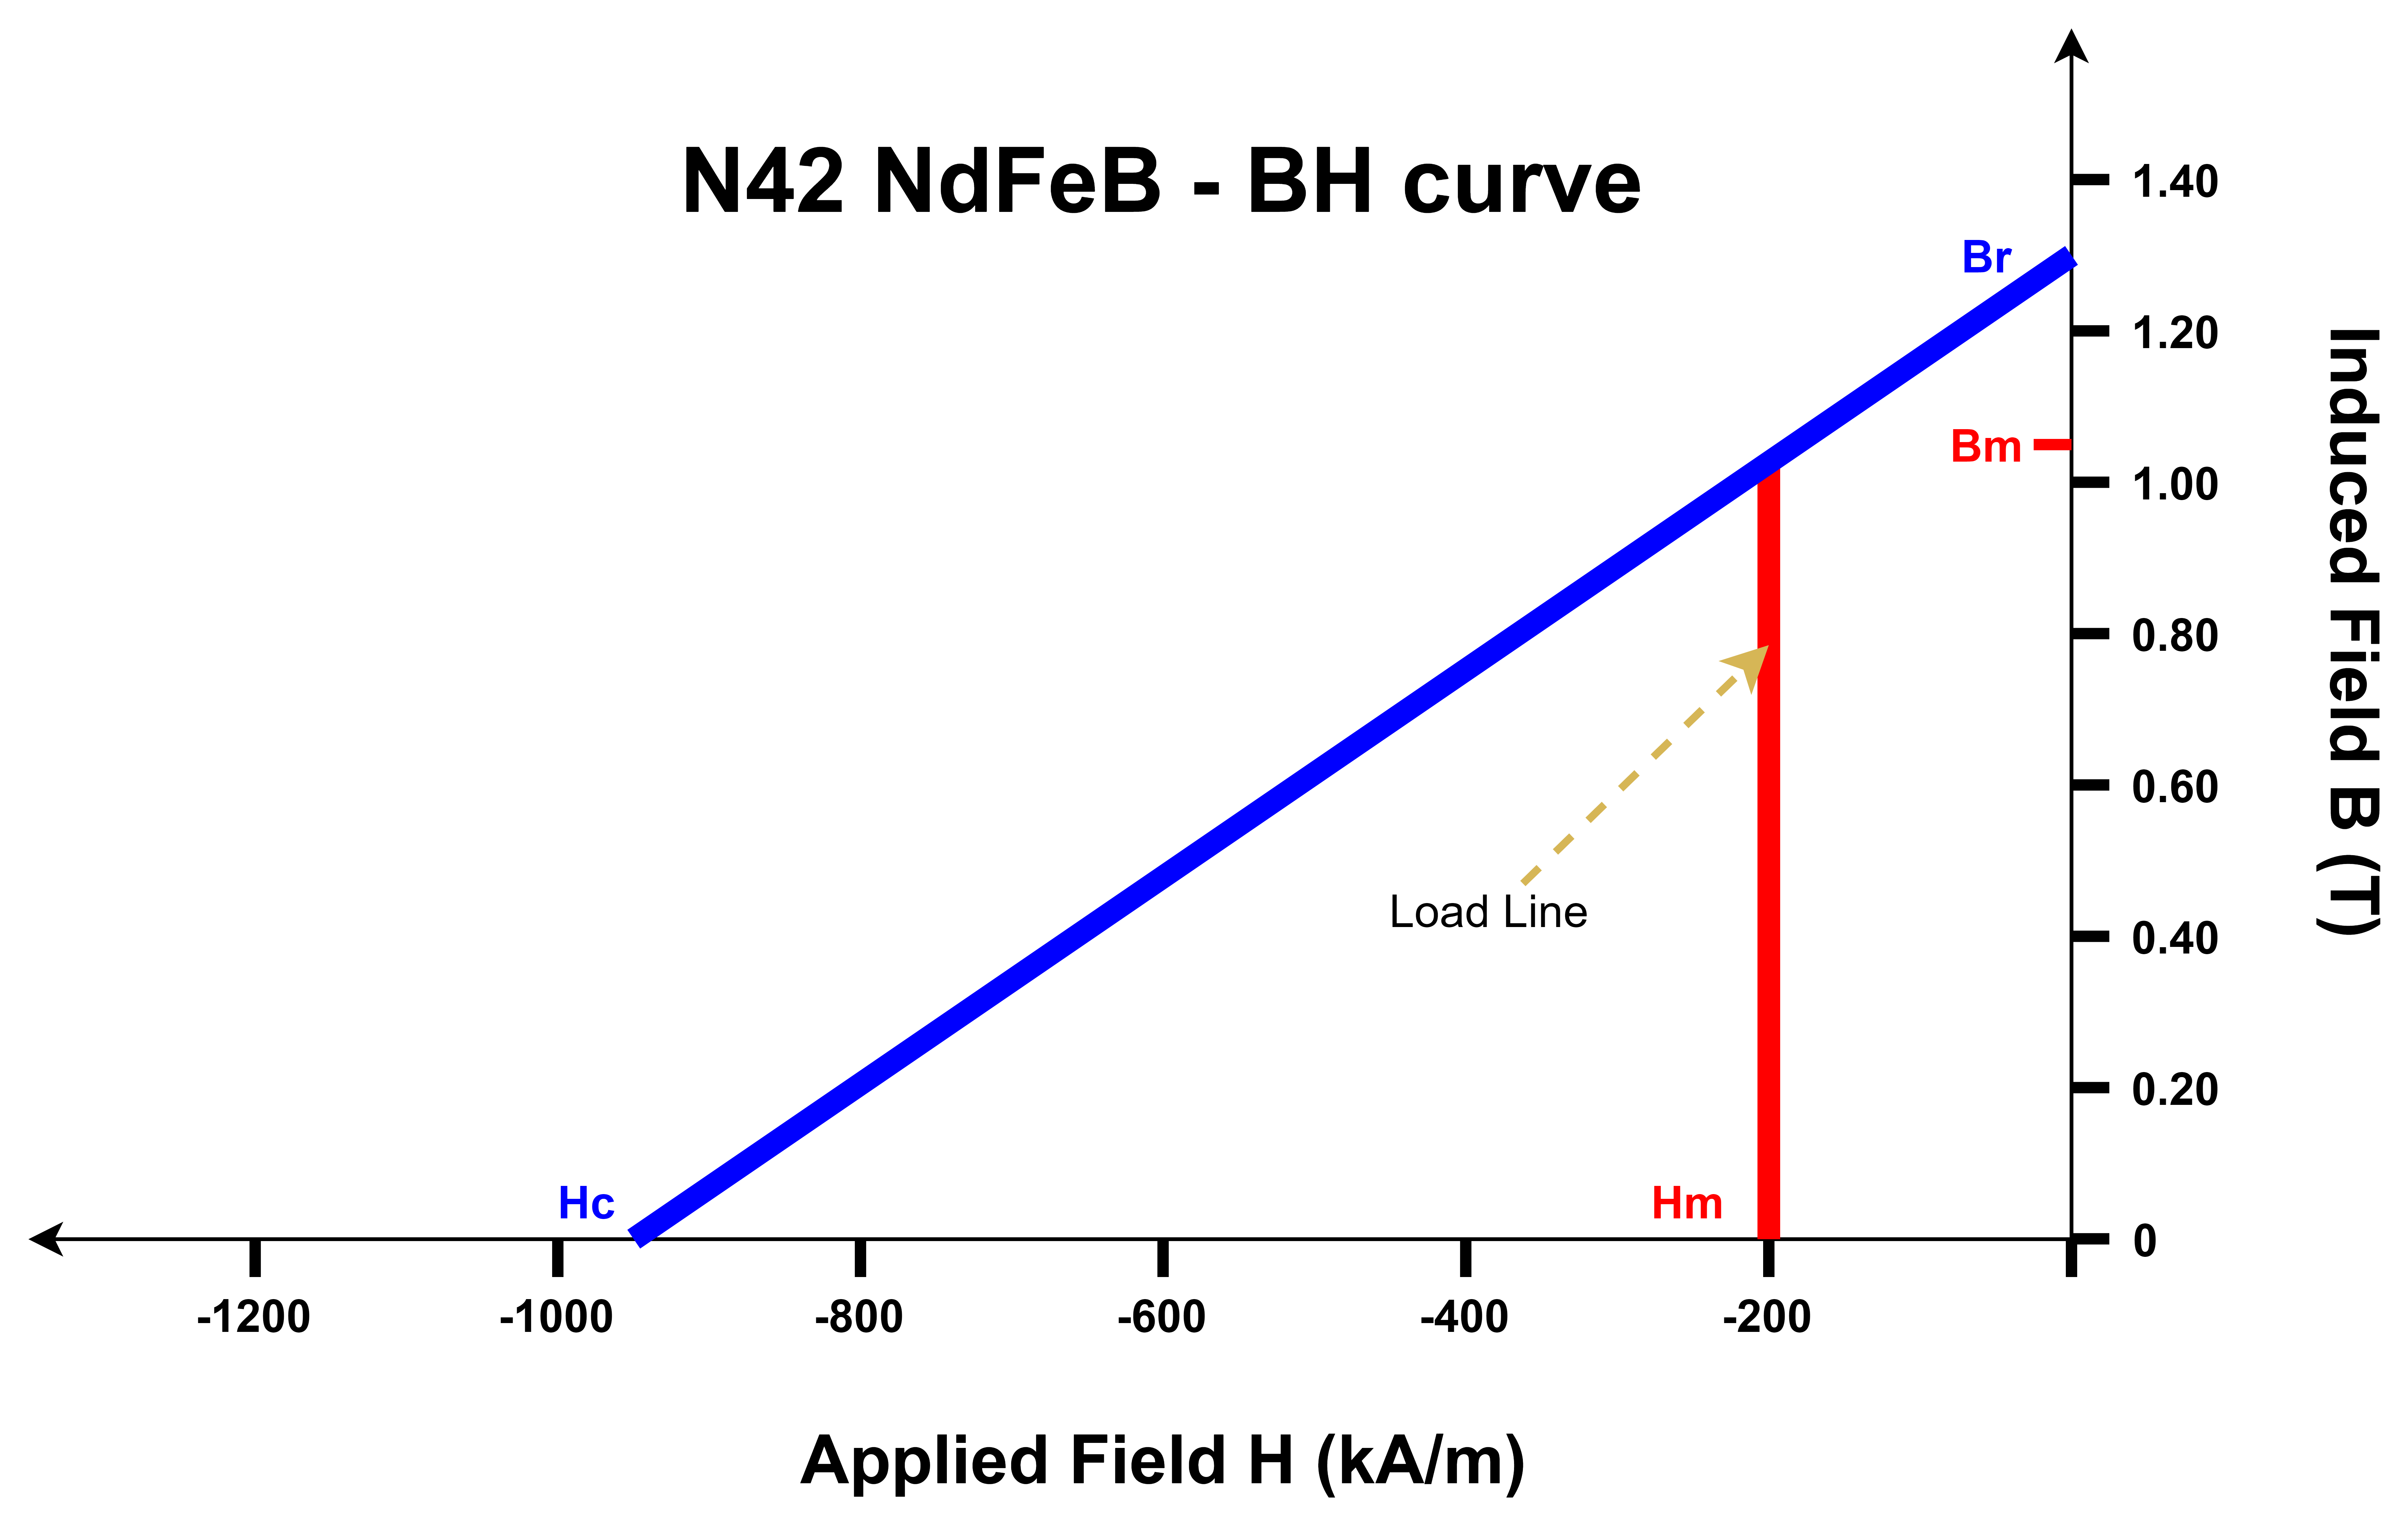
\includegraphics[scale=0.8]{Figures/BHCurve.png}
\caption{N42 NdFeB - BH curve with load line}
\label{fig:BHCurve}
\end{figure}

\begin{figure}[h!]
\centering
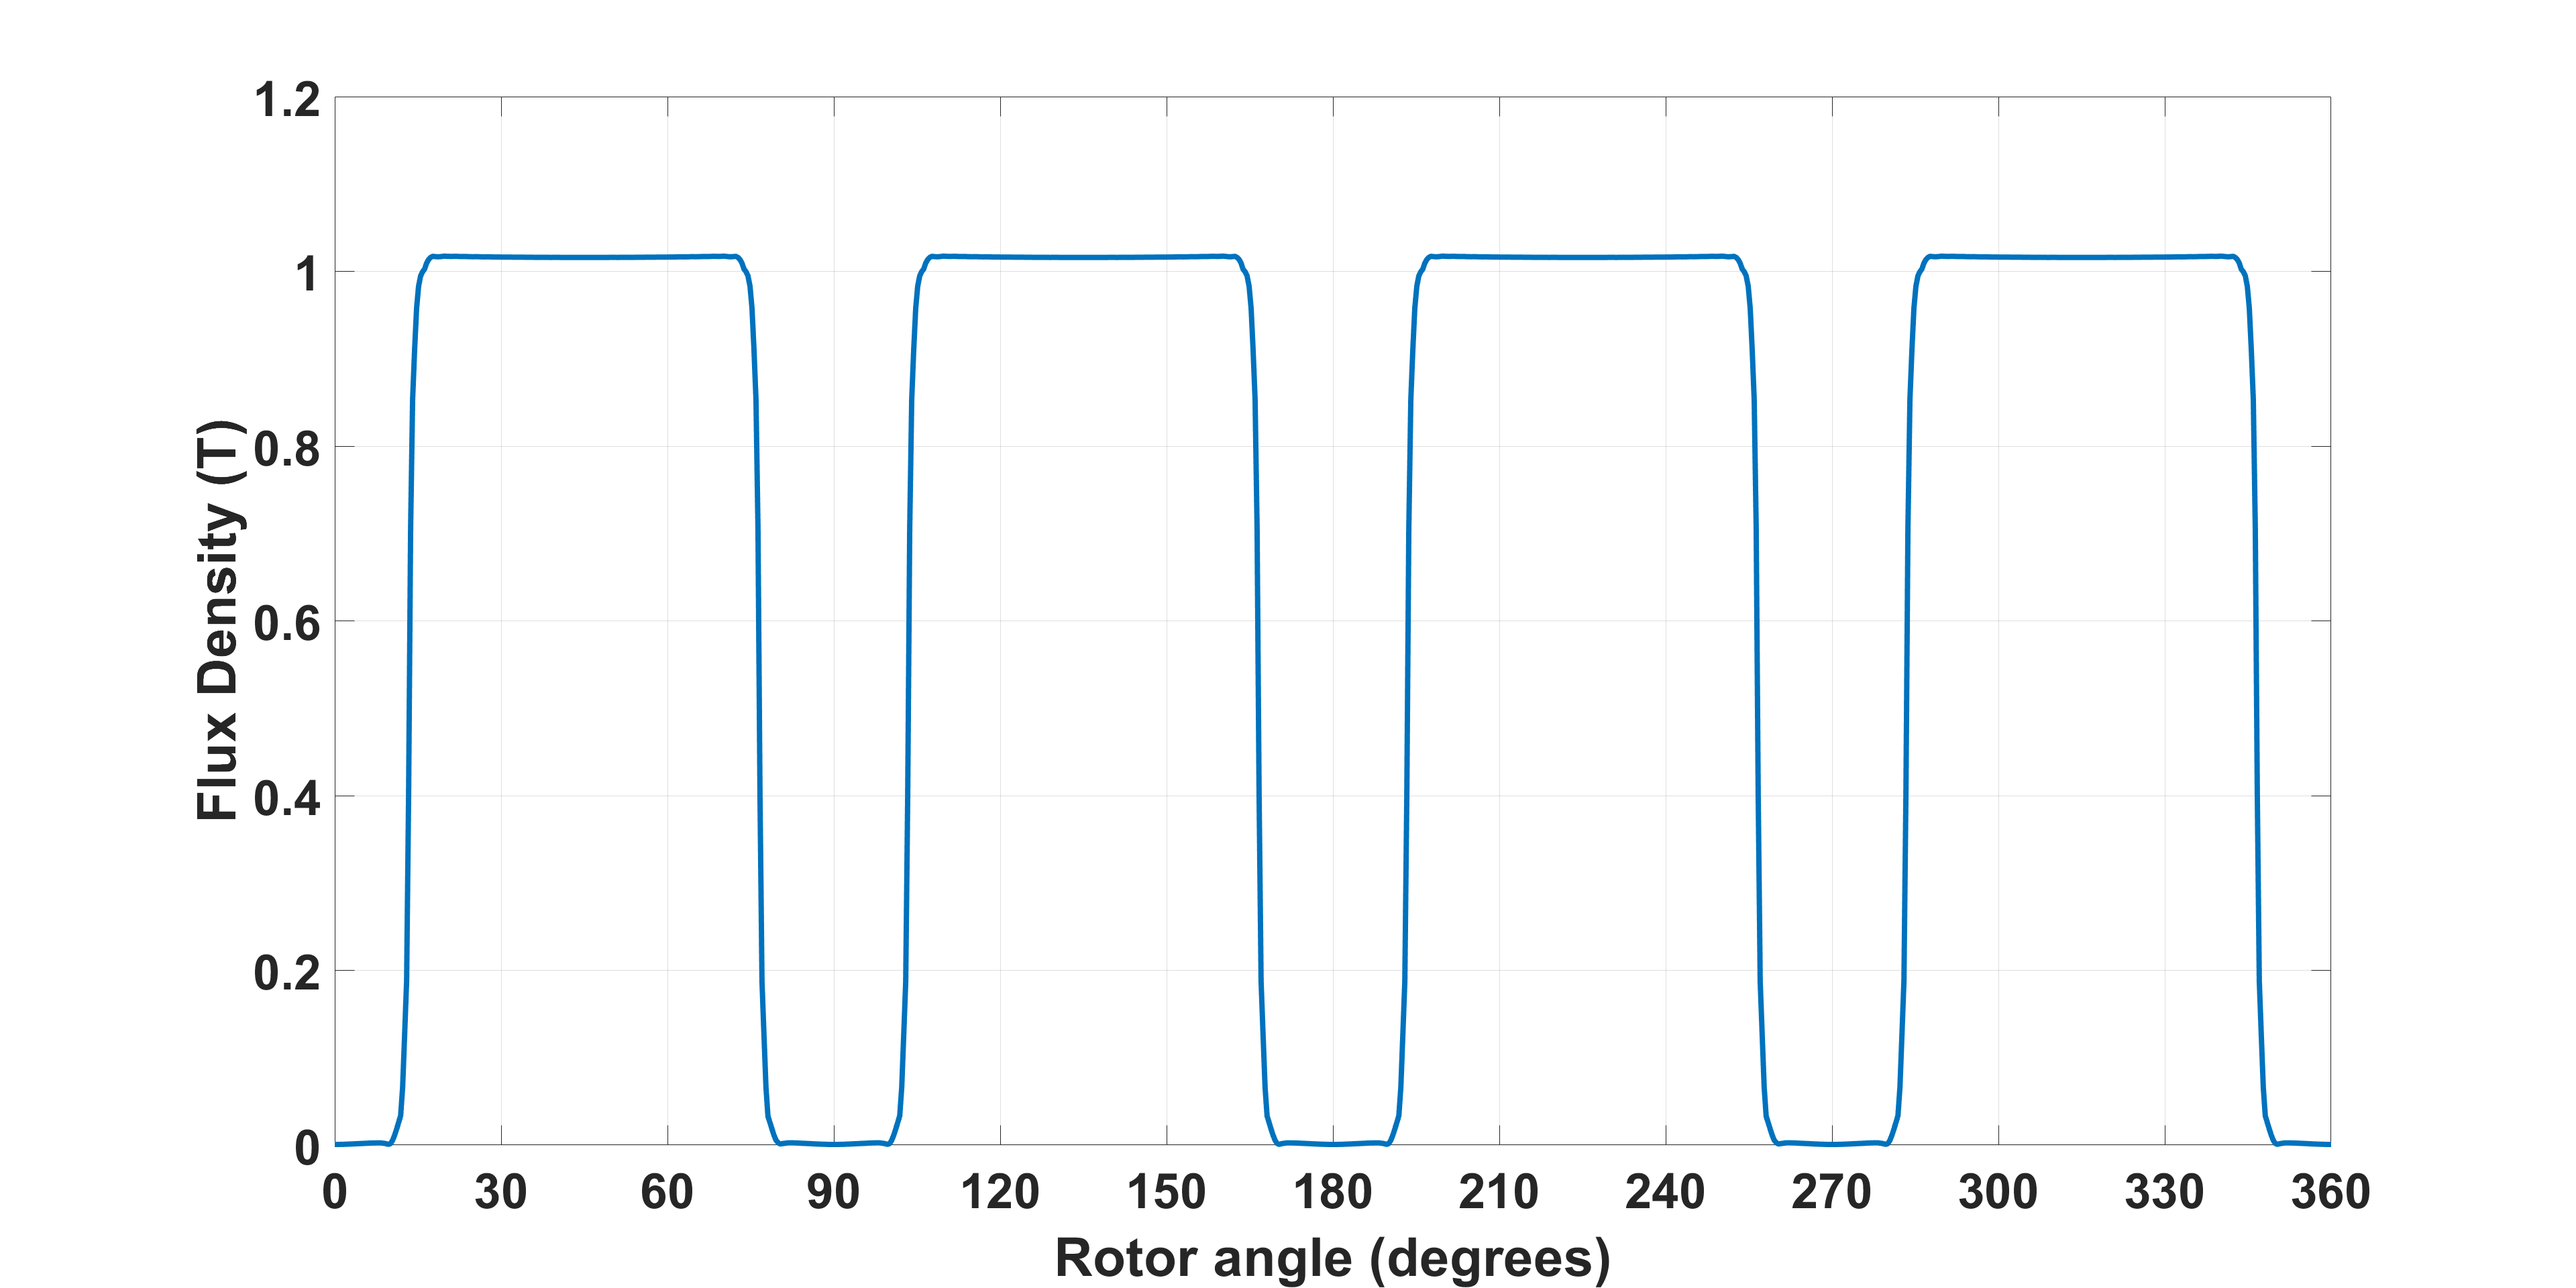
\includegraphics[scale=0.15]{Figures/MagB.png}
\caption{Magnetic Flux Density Magnitude }
\label{fig:MagB}
\end{figure}

\section{Question 2 - Electrical Loading and Machine Sizing}
\subsection{Part - a}
The number of slots are chosen to be 36, which gives out a reasonable slot width value of $4.363 \: \mathrm{mm}$ as calculated in (\ref{eqn:SlotWidth}). Moreover the distribution factors for the chosen number of slots are listed in Table \ref{table:WindingFactor}. The winding factors for the harmonic could be reduced using a different number of slots, which is out of the scope of this study. 



\begin{equation} \label{eqn:SlotWidth}
    W_{Slot} = \frac{\pi \cdot D_i}{2 \cdot N_{slot}} =  4.363 \: \mathrm{mm}
\end{equation}
\begin{table}[h!] 
\begin{center}
\caption{Winding Factors for the chosen slots}
\label{table:WindingFactor}
\begin{tabular}{ |p{3cm}||p{3cm}|p{3cm}|p{3cm}|  }
 \hline
  Harmonic order: & First	& Third &Fifth\\
 \hline
 kd	& $0.96$	&	$0.64$ & $0.192$\\
 \hline
 kp &	$1$	& $-1$	&$1$\\
 \hline
 kw &$0.96$	& $-0.64$&	$0.192$\\
  \hline
 \end{tabular}
 \end{center}
 \end{table}

 \subsection{Part - b}
 For $2.5 \: \mathrm{A_{rms}}$ current and $5 \: \mathrm{\frac{A}{mm^2}}$ current density, the required wire area is calculated in (\ref{eqn:CopperArea}). For the calculated copper wire area, AWG20 cable is chosen whose area and diameter are $0.518 \: \mathrm{mm^2}$ $0.406 \: \mathrm{mm}$ respectively.

\begin{equation} \label{eqn:CopperArea}
    A_{wire} = \frac{2.5 \: \mathrm{A_{rms}}}{5 \: \mathrm{\frac{A}{mm^2}}} =  0.5 \: \mathrm{mm^2}
\end{equation}

\subsection{Part - c}
It is known that the optimal torque value is obtained when slot ratio value is $\frac{1}{\sqrt{3}}$. Therefore, the slot ratio is chosen as $0.6$. Considering the slot ratio, The slot-end diameter and the height of the slots are calculated in (\ref{eqn:SlotHeight}). 

The back core thickness is chosen for a peak flux density value of 1.5 Tesla. The resultant stator outer diameter is provided in (\ref{eqn:StatorOuterDiameter}).

\begin{equation} \label{eqn:SlotEndDiameter}
    D_{SlotEnd} = \frac{D_i}{\mathrm{Slot \: Ratio}} = 166.67 \: \mathrm{mm};
\end{equation}
\begin{equation} \label{eqn:SlotHeight}
    H_{Slot} = \frac{\mathrm{D_{slotend}-D_i}}{2} = 33.33 \: \mathrm{mm}
\end{equation}
\begin{equation} \label{eqn:BackCoreDepth}
    H_{BackCore} = \frac{\phi_{pp}}{\hat{B}_{airgap} \cdot L_{axial}} = 42.6 \: \mathrm{mm}
\end{equation}
\begin{equation} \label{eqn:StatorOuterDiameter}
    D_{o} = \mathrm{D_{slotend}} + 2\cdot H_{backcore}= 251.9 \: \mathrm{mm}
\end{equation}

\subsection{Part - d}
In order to calculate the electrical loading, number of turns per slot must be calculated. To calculate the number of turns, fill factor value is chosen as $\pmb{0.5}$. Note that, the fill factor is chosen relatively low for thermal consideration but may need further iteration. The calculation of the number of turns is provided in \ref{eqn:NumberOfTurnsPerSlot}.

\begin{equation} \label{eqn:NumberOfTurnsPerSlot}
    N_{turn} = \frac{H_{slot} \cdot W_{slot} \cdot FillFactor}{A_{AWG20}} \approx 141 \: \frac{\mathrm{turns}}{\mathrm{slot}}
\end{equation}


The electrical loading of the machine is provided in \ref{eqn:ElectricalLoading}. The current value was stated as $2.5 \: A_{rms}$. 
\begin{equation} \label{eqn:ElectricalLoading}
    A_{rms} = \frac{N_{turn} \cdot I_{rms} \cdot N_{slot}}{\pi \cdot \: D_i} = 40393.52 \: \mathrm{\frac{\mathrm{A}}{\mathrm{m}}}
\end{equation}



The obtained $40.4 \frac{\mathrm{kA}}{m}$ value is in the reasonable range which is between $35-65 \frac{\mathrm{kA}}{\mathrm{m}}$.

\subsection{Part - e}
The peak airgap flux density is found as $1.0174\: \mathrm{T} $ from the FEA results. The resultant average tangential stress and total force are provided in (\ref{eqn:AverageStress}) and (\ref{eqn:TotalForce}) respectively.
\begin{equation} \label{eqn:AverageStress}
    \sigma_{tan} = \frac{A_{rms} \cdot \hat{B} \cdot cos(\phi)}{\sqrt{2}} = 29059.81 \: \mathrm{Pa}
\end{equation}
\begin{equation} \label{eqn:TotalForce}
    F = \sigma_{tan} \cdot \pi \cdot D_i \cdot \L_{axial} = 912.94 \: \mathrm{Newton}
\end{equation}
\begin{equation} \label{eqn:Torque}
    T = \frac{F \cdot D_i}{2} = 45.65 \: \mathrm{Nm}
\end{equation}

\subsection{Part - f}
At a rated speed of 1500 rpm, the power of the machine can be calculated in (\ref{eqn:Power}).

\begin{equation} \label{eqn:Power}
    P = T \cdot \omega  = 7.17 \: \mathrm{kW}
\end{equation}




% \begin{equation} \label{eqn:CopperRadius}
%    R_{copper} = \sqrt{\frac{A_{wire}}{\pi}} =  0.5 \: \mathrm{mm^2}
%\end{equation}
%
%
% Memoization
\bibliographystyle{plain}
\bibliography{references}
\end{document}